% Niveau :      PCSI *
% Discipline :  Chimie Orga I
% Mots clés :   Spectrométrie UV-visible, Réactions acidobasiques

\begin{exercise}{Méthode de Gran}{2}{PCSI}
{Chimie générale,Réactions acidobasiques,Gran (méthode de),Titrage}{bermu}

\begin{questions}
\questioncours Allure du graphe d'un titrage d'un volume $v_\text{a}$ d'acide faible AH de concentration $c_\text{a}$ par une base forte $\mathrm{OH^-}$ de concentration $c_\text{b}$. \\
On définira les notions utilisées et on donnera un acide faible et une base forte comme exemples.

\question\label{qu:eqi} Définir l'équivalence et décrire les méthodes permettant de repérer l'équivalence et leurs limites. \\
Donner la relation entre $v_\text{eq}$, $v_\text{a}$, $c_\text{a}$ et $c_\text{b}$.

\begin{EnvUplevel}
    Nous allons étudier une méthode graphique permettant de repérer l'équivalence de ce titrage par suivi pH-métrique : la méthode de Gran.
\end{EnvUplevel}

\question \'Ecrire la réaction acidobasique prépondérante en jeu dans ce titrage et justifier qu'elle puisse être considérée comme totale.

\uplevel{On se place tout d'abord \underline{avant l'équivalence} $v_\text{b} < v_\text{eq}$.}

\question\label{qu:tab} \'Ecrire le tableau d'avancement de la réaction acidobasique à l'aide de $c_\text{a}$, $c_\text{b}$, $v_\text{b}$ et $v_\text{eq}$.

\question Rappeler la relation d'Henderson--Hasselbalch entre pH, p$K_\text{a}$, $\mathrm{[A^-]}$ et $\mathrm{[AH]}$, et déduire de la question précédente la relation suivante : \vspace{-.5em}
$$V_1 \equiv v_\text{b} 10^{\text{p}K_a-\text{pH}} = v_\text{eq} - v_\text{b}.\vspace{-1em}$$

\uplevel{On se place maintenant \underline{après l'équivalence} $v_\text{b} > v_\text{eq}$.}

\question Reprendre le cheminement de la question \ref{qu:tab}\,et en déduire la relation suivante : \vspace{-.5em}
$$V_2 \equiv (v_\text{b} + v_\text{a}) 10^{\text{pH}_{\,}-\text{pH}_\text{b}} = v_\text{b} - v_\text{eq}, \vspace{-.8em}$$
où $\text{pH}_\text{b}$ désigne le pH de la solution de base forte.

\question Interpréter le graphe ci-dessous ($c_b = 10^{-2}$ M, $v_a = 10$ mL) : \vspace{-1.2em}

\begin{EnvUplevel}
    \begin{figure}[H]
        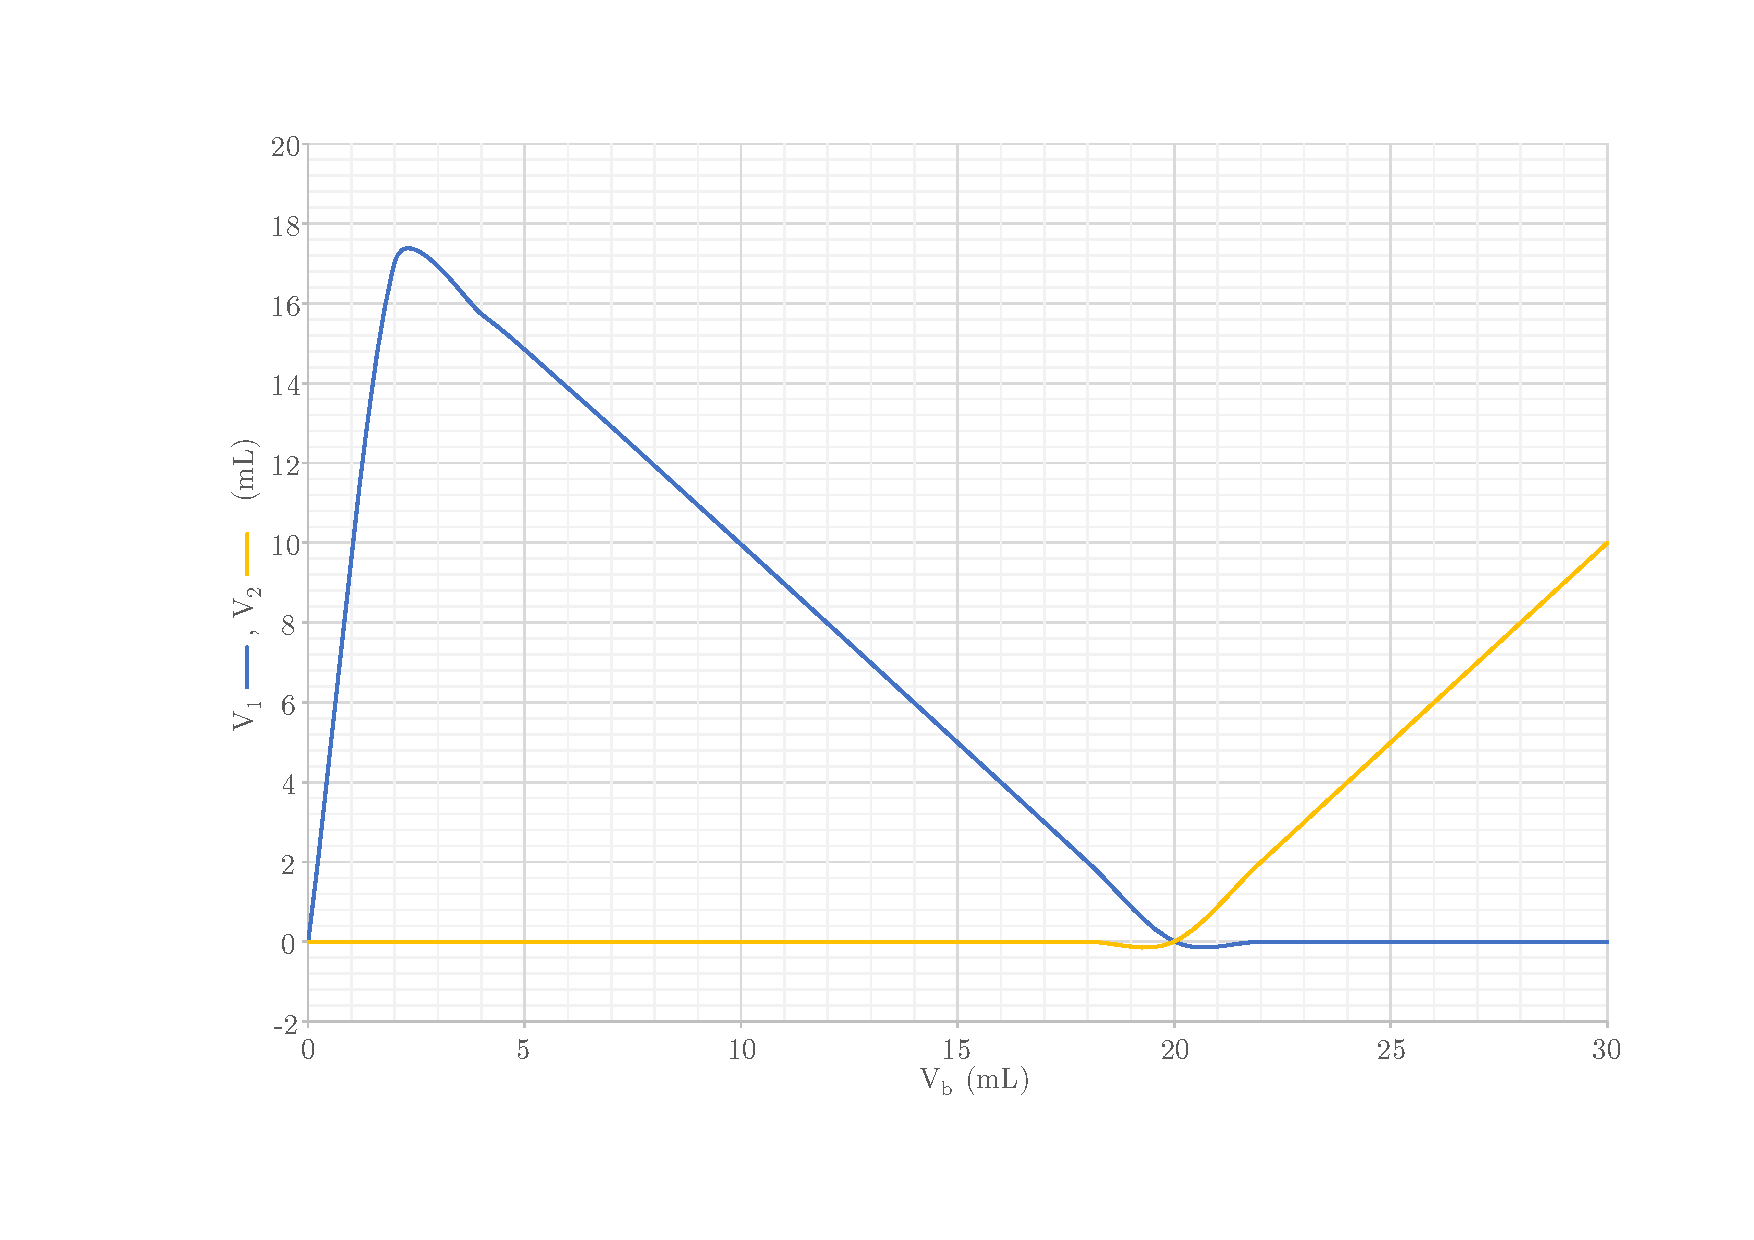
\includegraphics[width=\linewidth]{chimie/pH/gran.pdf}
        \caption{Graphe de Gran du dosage d'un acide faible par une base forte.}
    \end{figure}\vspace{-1.2em}
\end{EnvUplevel}

\question Commenter la zone $v_b\in [0 ; 2]$ mL.

\question Quels sont les avantages de la méthode de Gran par rapport à celles de la \ref{qu:eqi}.

\end{questions}
\end{exercise}

\begin{solution}
\begin{questions}
    \questioncours
    \begin{center}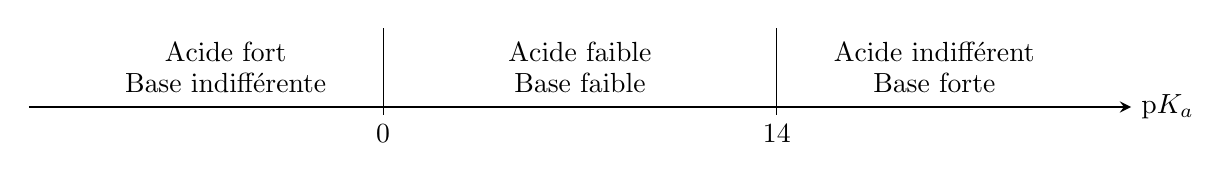
\begin{tikzpicture}[baseline=1em]
        \draw[->, >=stealth, thick] (-7,0)--(7,0) node[right]{p$K_\text{a}$};
        \draw[black] (-2.5,1)--(-2.5,-0.1) node[below]{0} ;
        \draw[black] (2.5,1)--(2.5,-0.1) node[below]{14} ;
        \node at (-4.5,.3) {Base indifférente};
        \node at (0,.3) {Base faible};
        \node at (4.5,.3) {Base forte};
        \node at (-4.5,.7) {Acide fort};
        \node at (0,.7) {Acide faible};
        \node at (4.5,.7) {Acide indifférent};
    \end{tikzpicture}\end{center}
    
    
    
    \question L'équivalence est le volume pour lequel on a introduit autant de quantité de titrant $n_\text{b}$ que de titré $n_\text{a}$
    $$n_\text{eq} = n_\text{a} = n_\text{b} \qquad \Longleftrightarrow \qquad c_\text{a} v_\text{a} = c_\text{b} v_\text{eq}.$$
    
    L'équivalence s'accompagne d'un saut de pH que l'on peut repérer par suivi pH-métrique ou grâce à un indicateur coloré, les limites de ces méthodes étant que la mesure de $v_\text{eq}$ est imprécise du fait de la largeur en volume du saut de pH qui peut être grande.
    
    \question La réaction est $\mathrm{AH + HO^- \leftrightharpoons A^- + H_2O}$. Elle a pour constante $10^{\text{p}K_\text{e} - \text{p}K_\text{a}} \gg 1$, d'où le fait qu'on puisse considérer qu'elle est totale.
    
    \question ~ \\[-2.5em]
    \begin{center}\begin{tabularx}{12cm}{r|C|C|C|C}
&
\multicolumn{1}{|c!{\makebox[0pt]{+}}}{AH}
&
\multicolumn{1}{c!{\makebox[0pt]{$\leftrightharpoons$}}}{OH$^-$}
&
\multicolumn{1}{c!{\makebox[0pt]{+}}}{A$^-$}
&
H$_2$O
\\
\hline\hline
Init. & $c_\text{a} v_\text{a}$ & $c_\text{b} v_\text{b}$ & $\varepsilon$ & $\infty$ \\
Fin. & $c_\text{a} v_\text{a} - c_\text{b} v_\text{b}$ & $\varepsilon$ & $c_\text{b} v_\text{b}$ & $\infty$ \\
& $ = c_\text{b}(v_\text{eq} - v_\text{b})$ & & & \end{tabularx}\end{center}
    
    \question Dans l'hypothèse où on se trouve dans le domaine d'Henderson, on a
    $$\text{pH} = \text{p}K_\text{a} + \log\mathrm{\dfrac{[A^-]}{[AH]}} = \text{p}K_\text{a} + \log\dfrac{\frac{c_\text{b}v_\text{b}}{v_\text{tot}}}{\frac{c_\text{b}(v_\text{eq} - v_\text{b})}{v_\text{tot}}},$$
    $$\text{d'où} \qquad v_\text{b} 10^{\text{p}K_a-\text{pH}} = v_\text{eq} - v_\text{b}.$$
       
    \question ~ \\[-2.5em]
    \begin{center}\begin{tabularx}{12cm}{r|C|C|C|C}
&
\multicolumn{1}{|c!{\makebox[0pt]{+}}}{AH}
&
\multicolumn{1}{c!{\makebox[0pt]{$\leftrightharpoons$}}}{OH$^-$}
&
\multicolumn{1}{c!{\makebox[0pt]{+}}}{A$^-$}
&
H$_2$O
\\
\hline\hline
Init. & $c_\text{a} v_\text{a}$ & $c_\text{b} v_\text{b}$ & $\varepsilon$ & $\infty$ \\
Fin. & $\varepsilon$ & $c_\text{b} v_\text{b} - c_\text{a} v_\text{a}$ & $c_\text{a} v_\text{a}$ & $\infty$ \\
 & & $ = c_\text{b}(v_\text{b} - v_\text{eq})$ & & \end{tabularx}\end{center}

    Cette fois-ci, c'est OH$^-$ qui impose sont pH. Ainsi,
    $$\text{pH} = \text{p}K_\text{e} + \log\dfrac{c_\text{b}(v_\text{b} - v_\text{eq})}{v_\text{a} + v_\text{b}}$$
    et donc en prenant en compte que pH$_\text{b} = \text{p}K_\text{e} + \log c_b$, on obtient
    $$(v_\text{b} + v_\text{a}) 10^{\text{pH}_{\,}-\text{pH}_\text{b}} = v_\text{b} - v_\text{eq}$$
    
    \question On retrouve bien les comportements de droite pour $V_1$ et $V_2$ au niveau de l'équivalence.
    
    Ici on déduit que $c_\text{a} = 2 \times 10^{-2}$ M.
    
    \question Initialement, l'hypothèse $\mathrm{[AH]}$ négligeable à l'équilibre n'est pas vérifiée car $c_\text{b} v_\text{b}$ est très petit et la réaction de dissociation de l'acide est donc prépondérante. La base réagit donc avec le H$_3$O$^+$ formé par AH.
    
    \question La méthode de Gran a pour avantage de repérer plus précisément l'équivalence mais elle repose sur des hypothèses fortes sur les composés titrés.
\end{questions}
\end{solution}